\documentclass{beamer}
\mode<presentation>
{
  %\usetheme{}
  %\usecolortheme{beaver}
  % 可供选择的主题参见 beameruserguide.pdf, 第 134 页起
  % 无导航条的主题: Bergen, Boadilla, Madrid, Pittsburgh, Rochester;
  % 有树形导航条的主题: Antibes, JuanLesPins, Montpellier;
  % 有目录竖条的主题: Berkeley, PaloAlto, Goettingen, Marburg, Hannover;
  % 有圆点导航条的主题: Berlin, Dresden, Darmstadt, Frankfurt, Singapore, Szeged;
  % 有节与小节导航条的主题: Copenhagen, Luebeck, Malmos, Warsaw
  %\setbeamercovered{transparent}
  % 如果取消上一行的注解 %, 就会使得被覆盖部分变得透明(依稀可见)
} 
\definecolor{kugreen}{RGB}{50,93,61}
\definecolor{kugreenlys}{RGB}{132,158,139}
\definecolor{kugreenlyslys}{RGB}{173,190,177}
\definecolor{kugreenlyslyslys}{RGB}{214,223,216}
\setbeamercovered{transparent}
\mode<presentation>
{  
  \usetheme{PaloAlto}
  \usecolortheme[named=kugreen]{structure}
  \useinnertheme{circles}
  \usefonttheme[onlymath]{serif}
  \setbeamercovered{transparent}
  \setbeamertemplate{blocks}[rounded][shadow=true]
}

\usepackage[english]{babel}
\usepackage{multirow}
\usepackage{amsmath}
\usepackage{amsfonts}
\usepackage{xkeyval}
\usepackage{graphics}
\usepackage{url}

\logo{
\includegraphics[scale=0.08]{images/HUSTLogo}}%Logo of the presentation
\title{Nonnegative Sparse PCA}  
\author{Yunfei Wang}
\institute{Department of Computer Science \& Technology \\ Huazhong University of Science \& Technology}
\date{\today} 

\begin{document}

\begin{frame}
\titlepage
\end{frame}


\begin{frame}\frametitle{Table of contents}\tableofcontents
\end{frame}


\section{Nonnegative Sparse PCA}
\subsection{PCA}
\begin{frame}\frametitle{PCA}
The decomposition performed by PCA is a linear combination of the input coordinates where the coefficients of the the principal vectors form a low-dimensional subspace that corresponds to the direction of maximal variance in the data.

\begin{equation}\label{eq:pca}
\begin{split}
&\max_U \frac{1}{2}\|U^TX\|_F^2=\max_U \frac{1}{2}Tr[U^TXX^TU]\\
&s.t.\; U^TU=I
\end{split}
\end{equation} 
PCA is attractive for a number of reasons.
\begin{itemize}
\item Maximum variance property provides a way to compress the data with minimal information loss.
\item Representation of the data in the projected space is uncorrelated.
\item PCA decomposition can be achieved via an eigenvalue decomposition of the data covariance matrix or SVD.
\end{itemize}
\end{frame}

\subsection{Nonnegative (Semi-Disjoint) PCA}
\begin{frame}\frametitle{Nonnegative (Semi-Disjoint) PCA}
Adding a nonnegativity constraint to PCA:
\begin{equation}\label{eq:npca1}
\begin{split}
&\max_U \frac{1}{2}\|U^TX\|_F^2\\
&s.t.\; U^TU=I,U\geq 0
\end{split}
\end{equation}
While disjoint principal component may be considered as a kind of sparseness, it is
too restrictive for most problems.We wish to allow some overlap among the principal vectors.$\parallel I-U^TU\parallel_F^2$ is typically used as a measure for orthonormality and the relaxed version of Eq(\ref{eq:npca1}) becomes,
\begin{equation}\label{eq:npca2}
\begin{split}
&\max_U \frac{1}{2}\|U^TX\|_F^2-\frac{\alpha}{4}\|I-U^TU\|_F^2\\
&s.t.\; U^TU=I,U\geq 0
\end{split}
\end{equation}
\end{frame}

\subsection{Nonnegative Sparse PCA(NSPCA)}
\begin{frame}\frametitle{Nonegative Sparse PCA(NSPCA)}
While semi-disjoint principal components can be considered sparse when the number of coordinates is small, it may be too dense when the number of coordinates highly exceeds the number of principal vectors. Minimizing the number of non-zero elements directly:
\begin{equation}\label{eq:nspca1}
\begin{split}
&\max_U \frac{1}{2}\|U^TX\|_F^2-\frac{\alpha}{4}\|I-U^TU\|_F^2-\beta\|U\|_{L_0}\\
&s.t.\;U\geq 0
\end{split}
\end{equation}
The $L_0$ norm could be relaxed by replacing it with a $L_1$ term
\begin{equation}\label{eq:nspca2}
\begin{split}
&\max_U \frac{1}{2}\|U^TX\|_F^2-\frac{\alpha}{4}\|I-U^TU\|_F^2-\beta\|U\|_{L_1}\\
&=\max_U \frac{1}{2}Tr[U^TXX^TU]-\frac{\alpha}{4}Tr[U^TUU^TU-2U^TU]\\
&\;\;\;-\beta 1^TU1-\frac{\alpha}{4}k\\
&s.t.\;U\geq 0
\end{split}
\end{equation}
\end{frame}

\subsection{Alogrithm}
\begin{frame}\frametitle{Algorithm of NSPCA}
The objective function of $u_{rs}$(the $r$ row and $s$ column of U) is:
\begin{equation}\label{eq:nspca2}
f(u_{rs})=-\frac{\alpha}{4}u_{rs}^4+\frac{c_2}{2}u_{rs}^2+c_1u_{rs}+const
\end{equation}
where const stands for terms that do not depend on $u_{rs}$.

Setting the derivative with respect to $u_{rs}$ to zero we obtain a cubic equation:
\begin{equation}\label{eq:derivative}
\frac{\partial f}{\partial u_{rs}}=-\alpha u_{rs}^3+c_2u_{rs}+c_1=0
\end{equation}
Evaluating Eq.(\ref{eq:nspca2}) for the nonnegative roots of Eq.(\ref{eq:derivative}) and zero, the nonnegative global maximum of $f(u_{rs})$ can be found.
\end{frame}

\begin{frame}\frametitle{How to find maximum?}
\begin{figure}
\begin{minipage}[b]{0.5\linewidth}
\centerline{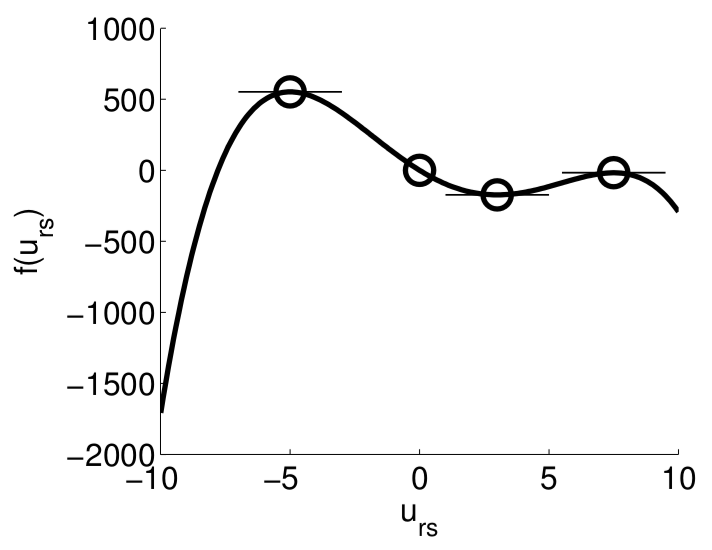
\includegraphics[scale=0.2]{images/pic1}}
\centerline{(a)4th order polynomial}  
\end{minipage}%
\hfill
\begin{minipage}[b]{0.5\linewidth}
\centerline{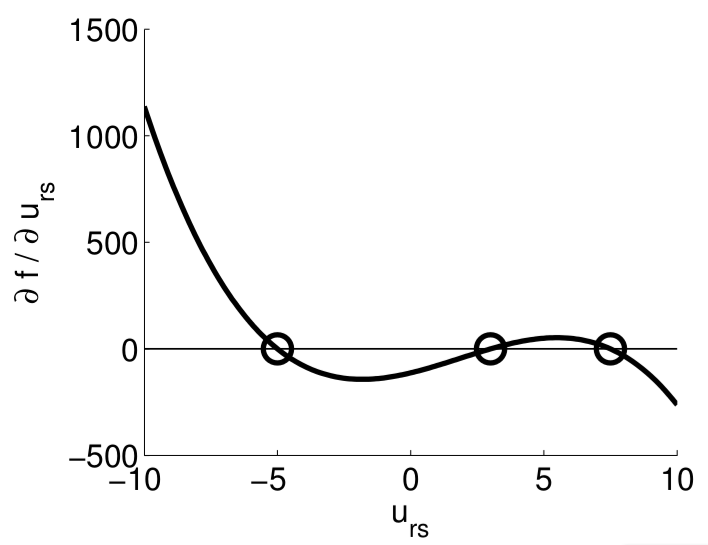
\includegraphics[scale=0.2]{images/pic2}}
\centerline{(b) corresponding derivative}
\end{minipage}
\end{figure}
In order to find the global nonnegative maximum, the function has to be inspected at all nonnegative extrema (where the derivative is zero) and at
$u_{rs}=0$.
\end{frame}


\section{Modifications on LSDA}
\begin{frame}\frametitle{Modifications on LSDA}
Generally,we project the data set $X=(\textbf{x}_1,\textbf{x}_2,\cdots,\textbf{x}_n)\in R^{n \times m}$ to $d$ directions and get a set of points $Y=(\textbf{y}_1,\textbf{y}_2,\cdots,\textbf{y}_n)^T\in R^{n \times d}$.

Objective function of within-class graph becomes:
\begin{equation}\label{eq:within}
\min Tr[Y^TL_wY]
\end{equation}

Objective function of between-class graph becomes:
\begin{equation}\label{eq:between}
\max Tr[Y^TL_bY]
\end{equation}

Objective function of sparseness becomes:
\begin{equation}\label{eq:sparse}
\min Tr[CY]
\end{equation}
where $C$ is a $d \times n$ matrix with all ones.

Constraint C: $Y \geq 0$
\end{frame}

\begin{frame}
Finally,we obtain our objective functions:
\begin{equation}\label{eq:objective}
\begin{split}
\min_Y F(Y)=&Tr[Y^TL_wY]-\alpha Tr[Y^TL_bY]+\beta Tr[CY]\\
&Tr[Y^T(L_w-\alpha L_b)Y]+\beta Tr[CY]
\end{split}
\end{equation}
\;\;\;$s.t. Y\geq 0$
\end{frame}

\begin{frame}
The curve of any element $Y_{rs}$ in $Y$ may have four possibilities:
\begin{figure}
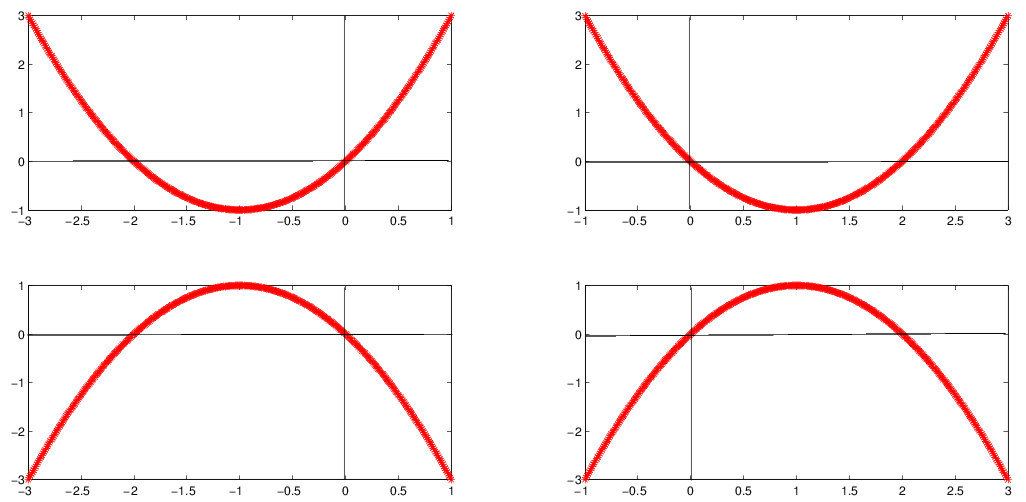
\includegraphics[scale=0.3]{images/plot}
\end{figure}
\end{frame}

\end{document}
